\section{Sophie Hatter}

\textbf{Name}: Sophie Hatter \\
\textbf{Function}: Hero, protagonist

\subsection{Internal World}

\textbf{Age \& Gender}: 19, Female \\
\textbf{Values \& Virtues}: Brave, loyal, friendly \\
\textbf{Personality}: Optimistic, intelligent, altruist, impulsive, compassionate \\
\textbf{Interests}: Hats, Magic \\
\textbf{Ethnic Group}: Human, Witch

\subsection{External World}
\textbf{Environment}: Wastelands, Howl’s Moving Castle \\
\textbf{Education}: Average-education \\
\textbf{Social \& Cultural Background}: Middle Class family \\
\textbf{Look \& Feel}: Her hair is white and looks like an old woman’s but she is a beautiful young girl. Generally she wears long dress. She loves to sew and wear hats \\
\textbf{Job \& Experience}: Cleaning woman, Hatter \\
\\
\textbf{Relatives \& Relation}:
\begin{enumerate}
\item \textbf{Howl}: She is in love with him, her partner. She lives with him in The Moving Castle with Calcifer
\item \textbf{Calcifer}: He his her friend and lives with her in The Moving Castle
\item \textbf{Justin}: Justin is her old friend who makes her meet Howl for the first time
\item \textbf{Suliman}: She respects Suliman as great magician and due to this fact she trusts her
\item \textbf{Mizar}: At the beginning she doesn’t know him. She is in conflict with her since she 
apprehends that Mizar has trapped Howl
\item \textbf{Belzel}: At the beginning she doesn’t know him. He is her last hope to rescue Howl from the reign of spirits
\end{enumerate}

\begin{figure}
\centering
\begin{subfigure}
  \centering
  
\includegraphics[scale=0.3]{Images/charactersColors}
\end{subfigure}
\begin{subfigure}
  \centering
  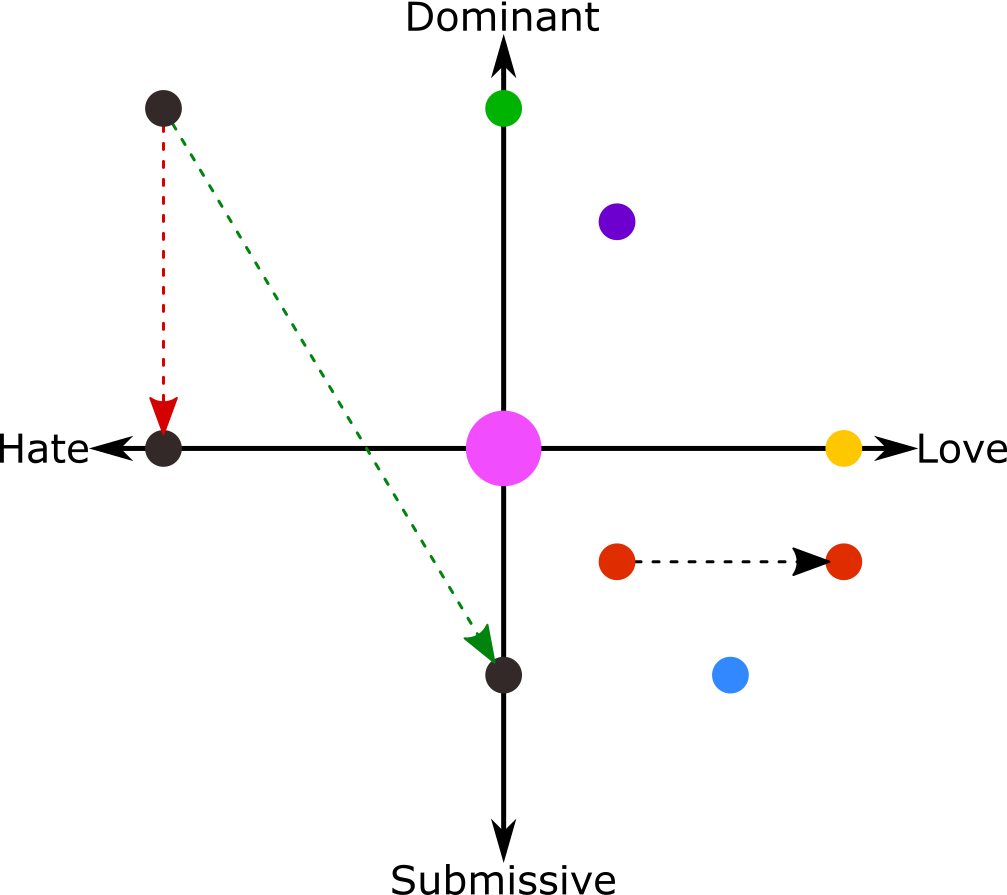
\includegraphics[width=8cm]{Images/Circumplexes/sophieCircumplex}
  \caption{Circumple of Sophie}
\end{subfigure}
\begin{subfigure}
  \centering
   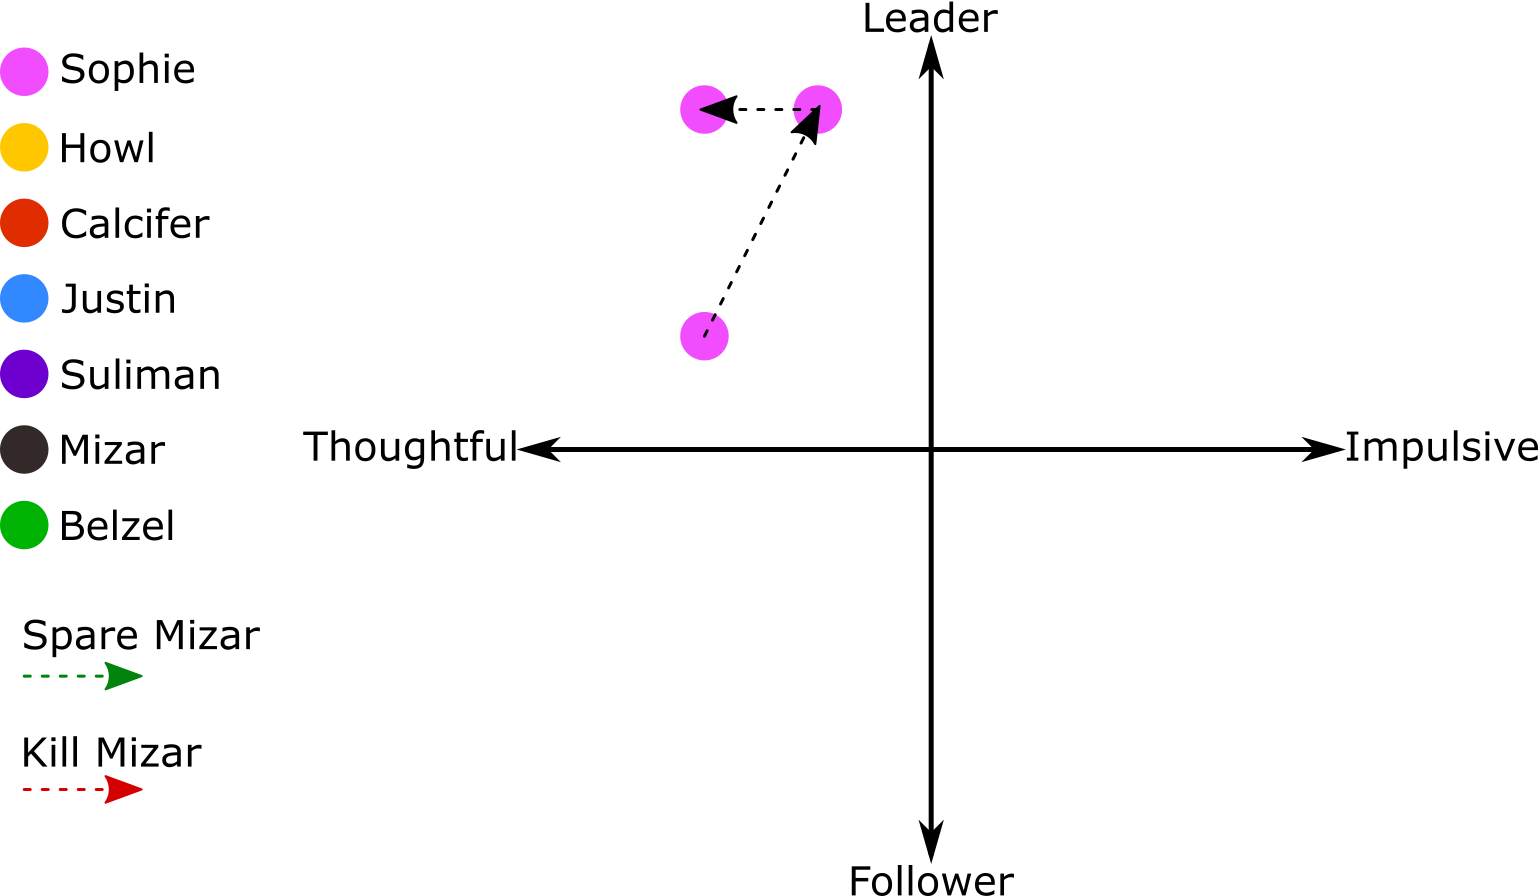
\includegraphics[width=8cm]{Images/Evolutions/sophieEvolution}
  \caption{Evolutions of Sophie}
\end{subfigure}
\end{figure}

\subsection{Description}
Sophie is brave and altruist girl. She represents the Hero of the Story who is going to save Howl. She is also optimistic but she always worries about her beloved ones. She hasn’t lost the passion for hats and occasionally she sews one.

\subsection{Background story}
Before She fell in love with Howl She lived in the small town within the Kingdom of Ingary. She is the eldest of two sisters and aimed to become a hatter like her father. After the misadventure of the curse launched by the Wastelands Witch, she has discovered being a which. Her white hair is the sign of the passed curse. Her magic powers lets her speak with some objects but she is a novice and she has to learn almost everything about the magic world.

